\section{Launcher}
Der Launcher ist ein eigenes Fenster, welches vor dem Öffnen der Benutzeroberfläche angezeigt wird. Hier hat der Benutzer die Möglichkeit eigene Profile zu erstellen, die Sprache zu ändern und sein Benutzerprofil zu starten. Auch werden hier die zuletzt geöffneten Profile anschaulich dargestellt.

\begin{figure}[h] 
  \centering
     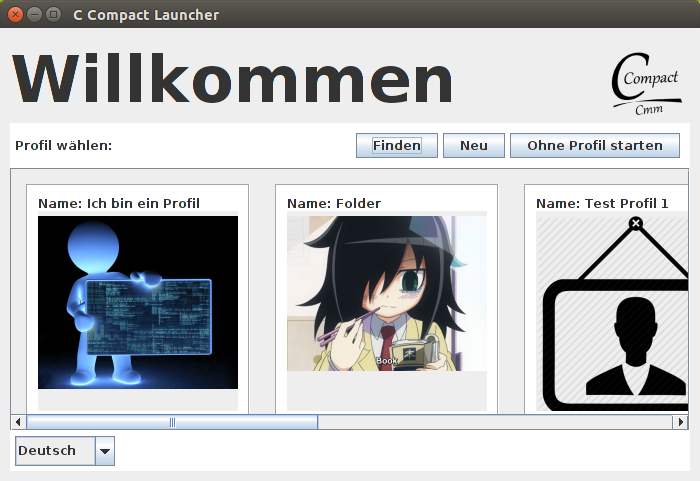
\includegraphics[width=0.9\textwidth]{./media/images/gui/launcher/launcher_main.png}
  \caption{Launcher GUI}
  \label{fig:Bild1}
\end{figure}

%TODO Verwei auf Anhang
Grundsätzlich ist der Launcher ein neues JFrame\footnote{\url{http://www.java-tutorial.org/jframe.html}}, das vor dem Start der Benutzeroberfläche angezeigt wird. Die zuletzt verwendeten Profile werden mithilfe einer JScrollpane\footnote{\url{http://www.java2s.com/Tutorial/Java/0240__Swing/CreatingaJTable.htm}}  , in welcher sich mehrere JPanels\footnote{\url{https://docs.oracle.com/javase/tutorial/uiswing/components/panel.html}} liegen, angezeigt. In den JPanels befinden sich der Name und das Benutzerbild.

\begin{itemize}
\item Falls kein letztes Profil vorhanden ist, wird auf die Erstellung eines neuen Profils hingewiesen.
\item Wenn der Benutzer kein Profilbild gewählt hat, wird ein voreingestelltes Profilbild verwendet.
\item Mit einem Klick auf das Profilbild kann das gewünschte Profil gestartet werden.
\item Es besteht die Möglichkeit C-Compact mithilfe des Launchers ohne Profil zu starten. Das bedeutet, dass kein Profil ausgewählt wurde und die Entwicklungsumgebung ohne dem Quest System gestartet wird.
\end{itemize}

\subsection{Erstellen eines neuen Profils}
Durch einen Klick auf den Button "`\textit{Neu}"' gelangt man in ein neues Fenster, indem man sein Profil erstellen kann.  

%TODO Anhang Referenzieren
Zuerst wird der Ordnerpfad mithilfe eines JFileChoosers [Kapitel: \ref{sec:JFileChooser}] abgefragt. Falls ein korrekter Pfad ausgewählt wurde, kann nun mithilfe einer JOptionPane\footnote{\url{http://docs.oracle.com/javase/7/docs/api/javax/swing/JOptionPane.html}} ein gewünschter Nutzername gewählt werden. 
\begin{lstlisting}[language=JAVA]
String name = JOptionPane.showInputDialog(null,
"Bitte Namen eingeben:",
 " Eingabeaufforderung",JOptionPane.PLAIN_MESSAGE);
p.setName(name);
\end{lstlisting}

Wenn die Eingabe erfolgreich war und nicht null ergeben hat, wird nun im gewählten ein neuer Ordner erstellt, welcher das Profil mit dem gewählten Namen repräsentiert. Darin befindet sich eine "`\textit{.cp}"' Datei, welche zum Öffnen ausgewählt werden kann. Sobald die Einstellungen vorgenommen wurden, wird die Entwicklungsumgebung mit dem neu gestalteten Profil gestartet.

Falls bei der Erstellung des Profils etwas schiefläuft oder abgebrochen wird, kommt man automatisch nach Anzeigen einer JOptionPane, welche eine Fehlermeldung beinhaltet, wieder zurück zum Launcher.

\subsection{Finden eines bereits existierenden Profils}
Damit ein Profil gestartet werden kann, welches nicht in den letzten Profilen im Launcher vorhanden ist, ist es notwendig, bereits existierende Profile finden zu lassen.

Sobald man auf den Button "`\textit{Finden}"' klickt, wird ein veränderter JFileChooser geöffnet. Hier kann nur eine "`\textit{.cp}"' Datei ausgewählt werden. Sobald diese angeklickt wurde, werden das Profilbild und der Profilname als Vorschau auf der rechten Seite angezeigt. Wenn der Nutzer kein Profilbild eingestellt hat, wird hier ein voreingestelltes Profilbild angezeigt.

\begin{figure}[h] 
   \centering
     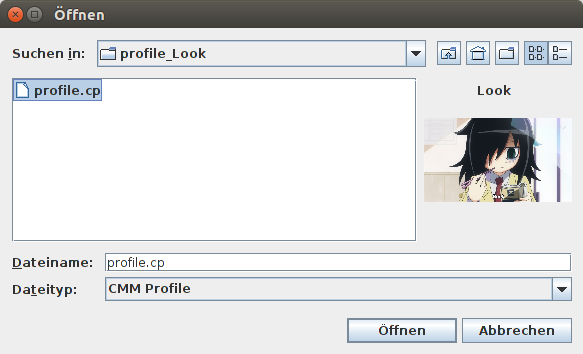
\includegraphics[width=0.9\textwidth]{./media/images/gui/launcher/launcher_finden.png}
  \caption{ Profilvorschau}
  \label{fig:Bild1}
\end{figure}

Wenn man nun weiter in der Ordnerstruktur auf der Suche ist, bleibt das Profil bereit zum Öffnen. Indem man auf den "`\textit{Öffnen}"'-Button klickt, startet man nun C-Compact mit dem gerade ausgewählten Profil und es wird automatisch zu den zuletzt verwendeten Profilen hinzugefügt.
